
\documentclass[10pt,a4paper]{article}
\usepackage[utf8]{inputenc}
\usepackage[T1]{fontenc}
\usepackage{geometry}
\geometry{margin=1in}
\usepackage{graphicx}
\usepackage{parskip}
\usepackage{titlesec}
\usepackage{xcolor}
\usepackage{enumitem}
\usepackage{hyperref}
\usepackage{fontawesome5}
\usepackage{setspace}
\usepackage{titling}

% Color settings
\definecolor{primary}{RGB}{0, 79, 144}
\definecolor{accent}{RGB}{50, 50, 50}
\definecolor{accentgray}{RGB}{90, 90, 90}
\definecolor{jobtitlegreen}{RGB}{0, 128, 96}  % Tealish green, modern and calm

% Section formatting
\titleformat{\section}
  {\Large\bfseries\color{primary}}{}{0em}{}
\titleformat{\subsection}[runin]
  {\bfseries\color{primary}}{}{0em}{}[.]

% Spacing between items
\setlist[itemize]{itemsep=4pt, topsep=4pt}

\hypersetup{
    colorlinks=true,
    linkcolor=primary,
    urlcolor=primary
}

\pagestyle{empty}

\geometry{
  top=1.5cm,
  bottom=1.8cm,
  left=2cm,
  right=2cm
}

\begin{document}

\vspace*{-1cm} % move header block closer to top of page

\noindent
\begin{minipage}[t]{0.65\textwidth}
    \textbf{\fontsize{24pt}{28pt}\selectfont Ryan Matthews}\\[0.2cm]
    \href{mailto:ryanjmatthews@gmail.com}{ryanjmatthews@gmail.com} \quad
    \href{https://linkedin.com/in/ryan-j-matthews}{LinkedIn} \quad
    \href{https://github.com/Darainer}{GitHub} \quad +49 176 34599887\\[0.6cm]
    \small
    \setstretch{1.8}
    Engineering leader with over 10 years of experience in automated driving development, delivering business outcomes in both technical and product leadership roles. Passionate about building commercially successful software and AI rich products.
\end{minipage}
\hspace{1.5cm}
\begin{minipage}[t]{0.25\textwidth}
    \raisebox{-\height}{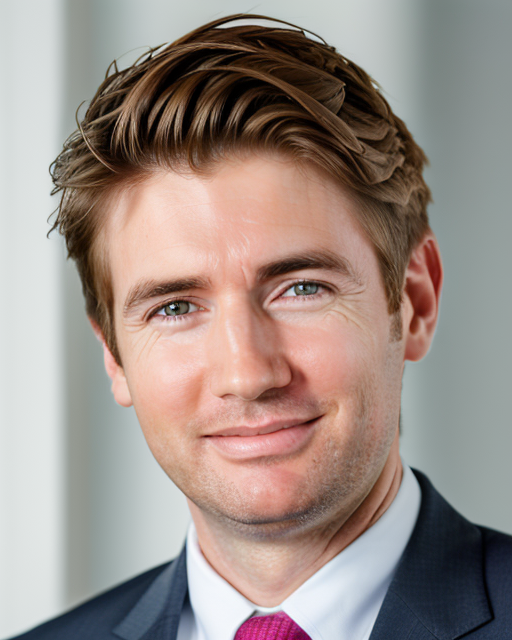
\includegraphics[width=\linewidth]{profile_pic_ryan.png}}
\end{minipage}


\vspace{1.2em}

% Work Experience
\section*{\textcolor{primary}{Work Experience}}

\subsection*{
  \textbf{\textcolor{jobtitlegreen}{Chief Architect ADAS/AD Applications}}, 
  \textcolor{gray}{\scshape Luminar} \hfill \textit{Jul 2022 – Present}
}
\begin{itemize}
    \item Reporting to the VP of Software, I provide hands-on technical direction across the Software, SoC, and Lidar product portfolio.
    \item Drove fundamental changes to software strategy in response to AI-centric ADAS market trends and our market position.
    \item Led software related pursuit activities in securing Luminar's first large software customer.
    \item Built and socialized a python / jupyter based toolchain for worldwide multidisciplinary product design.
\end{itemize}

\subsection*{
    \textbf{\textcolor{jobtitlegreen}{Product Owner Active Safety}}, 
    \textcolor{gray}{\scshape Luminar} \hfill \textcolor{primary}{\textbf{\textit{{Sep 2020 – Jun 2022}}}}
}
\begin{itemize}
    \item Led Development of a NCAP 2023-compliant Lidar-only active safety product
    \item Successfully demonstrated to leading automaker CEOs and industry icons at \href{https://ces.tech}{CES 2022} and \href{https://www.iaa-mobility.com}{IAA 2022}
    \item Built and mentored a high-performing ADAS development team including my successor.
\end{itemize}

\subsection*{
    \textbf{\textcolor{jobtitlegreen}{Product Owner ADAS}}}, 
    \textcolor{gray}{\scshape Samsung Electronics} \hfill \textcolor{primary}{\textbf{\textit{{Apr 2019 – Sep 2020}}}}
\begin{itemize}
    \item Led camera-only AEB NCAP 2022+ product development as the first ever safety critical application of a Samsung System on a Chip.
    \item Directed algorithm development SoC design to meet application requirements and safety standards.
\end{itemize}

\subsection*{\textbf{\textcolor{jobtitlegreen}{Senior Developer}}}, 
    \textcolor{gray}{\scshape Zenuity (Volvo / Autoliv Joint Venture)} \hfill \textcolor{primary}{\textbf{\textit{{Mar 2018 – Mar 2019}}}}
\begin{itemize}
    \item Migrated codebase to utilize a modern CI/CD environment and introduced data-driven development practices.
    \item Achieved milestone of having nightly functional KPI evaluations to validate any changes on a world-wide driving dataset.
\end{itemize}

\subsection*{\textbf{\textcolor{jobtitlegreen}{Lead Feature Developer}}}, 
    \textcolor{gray}{\scshape Autoliv Electronics} \hfill \textcolor{primary}{\textbf{\textit{{Oct 2016 – Mar 2018}}}}
\begin{itemize}
    \item Developed tracking/control algorithms for novel camera-only automated driving.
    \item Patented technology, Major camera program wins, successful integration with partners.
\end{itemize}

\subsection*{\textbf{\textcolor{jobtitlegreen}{Engineering Consultant}}}, 
\textcolor{gray}{\scshape TESIS DYNAware, Munich} \hfill \textcolor{primary}{\textbf{\textit{{Feb 2011 – Sep 2016}}}}
\begin{itemize}
    \item Managed software projects exceeding \$1M budget with >10-person teams.
    \item Delivered ADAS and ESP algorithms to Tier 1s and German OEMs.
\end{itemize}

\subsection*{\textbf{\textcolor{jobtitlegreen}{Mechatronic Engineer}}}, 
\textcolor{gray}{\scshape Australian Submarine Corporation, Perth} \hfill \textcolor{primary}{\textbf{\textit{{Jan 2007 – Apr 2010}}}}
\begin{itemize}
    \item Designed and supported submarine control systems on active submarines.
\end{itemize}

\vspace{1.2em}

% Education
\section*{Education}

\textbf{B.Eng (Hons), Mechatronic Engineering}, University of Adelaide \\
\textit{First Class Honours, Dean's List, Aerospace Project Award} \\[4pt]
\textbf{Bachelor of Economics}, University of Adelaide \\
\textit{Major in mathematical modelling and statistics}

\vspace{1.2em}

% Relevant Skills
\section*{Relevant Skills}

\begin{minipage}[t]{0.48\textwidth}
    \textbf{\textcolor{primary}{Software Development}}
    \begin{itemize}
        \item C++
        \item Python
        \item Model based development
    \end{itemize}
\end{minipage}
\hfill
\begin{minipage}[t]{0.48\textwidth}
    \textbf{\textcolor{primary}{Standards / Processes}}
    \begin{itemize}
        \item Functional Safety ISO 26262
        \item SOTIF ISO 21448
        \item AUTOSAR C++ 14
    \end{itemize}
\end{minipage}

\vspace{1.2em}

% Further Education
\section*{Further Education}

\begin{itemize}
    \item \textbf{Nov 2024}: Deep learning Specialization (\href{https://www.deeplearning.ai}{Deeplearning.ai})
    \item \textbf{Sep 2023}: Creative leadership certificate (18 month program \href{https://mvr.de}{mvr.de})
    \item \textbf{July 2022}: Modern C++ training (\href{https://klaus-iglberger.com}{Klaus Iglberger})
    \item \textbf{Apr 2020}: Advanced modern C++ training program (\href{https://nicolaijosuttis.com}{Nicolai Josuttis})
    \item \textbf{Feb 2020}: Professional Scrum Product Owner (\href{https://scrum.org}{scrum.org})
    \item \textbf{Nov 2017}: Certified Scrum Master (\href{https://scrumalliance.org}{Scrum Alliance})
    \item \textbf{Jul 2015}: MathWorks Certified MATLAB Associate (\href{https://www.mathworks.com}{MathWorks})
    \item \textbf{Dec 2014}: Certified Project Management Professional (\href{https://www.pmi.org}{PMP}\textsuperscript{\textregistered})
\end{itemize}

\vspace{1.2em}

% Languages

\section*{Languages}
English (Native), German (Full Professional)

\end{document}
